\chapter{Sparse Kernel Machines}
\label{chap:Sparse Kernel Machines}
\section{Introduction}
One of significant limitations of kernel methods is that the kernel function $\mathcal{k}(\vec{x}_n,\vec{x}_m)$ must be evaluated for all possible pairs $\vec{x}_n$ and $\vec{x}_m$ of training points,computationally infeasible.Kernel-based algorithms that have \textbf{sparse} solutions predict for new inputs depend only on the kernel function evaluated at a subset of the training data points,such as \textbf{suport vector machine}(SVM).
\section{Maximum Margin Classifiers}
Two-class classification problem using linear models
\begin{align}
y(x) = \vec{w}^T\phi(x)+b
\end{align}
where $\phi(x)$ denotes a fixed feature-space transformation,and $b$ is bias parameter.

For linear separable feature space,the parameters satisfies $y(\vec{x}_n)>0$ for points having $t_n=+1$ and $y(\vec{x}_n)<0$ for $t_n=-1$,so that $t_ny(\vec{x}_n)>0$ for all points.

\textbf{Margin} is the smallest distance between the decision boundary and any of the samples.The maximum margin solution can be motivated using \textbf{computational learning theory},also known as \textbf{statistical learning theory}.
\begin{figure*}

	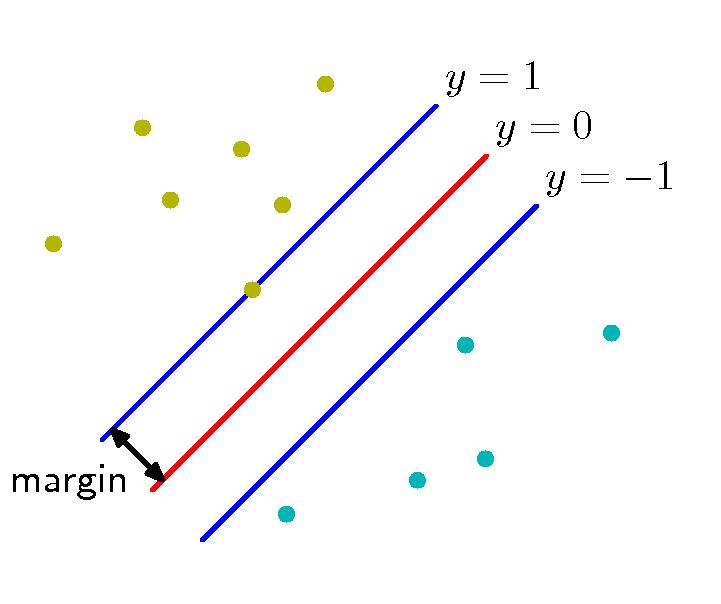
\includegraphics{prml/Figure7.1a.jpg}
	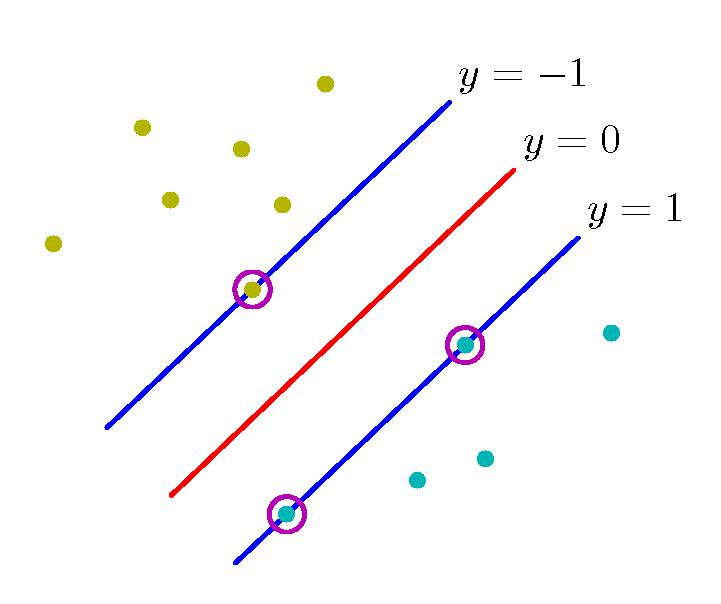
\includegraphics{prml/Figure7.1b.jpg}
	\caption{margin}
\end{figure*}

The \textbf{funtional margin} $t_ny(\vec{x}) > 0$ for data points correctly classified.The maximize it
\begin{align}
\vec{w},b = \arg\max\limits_{\vec{w},b}\{\dfrac{1}{\parallel\vec{w}\parallel}\min_n
[t_n(\vec{w}^T\phi(\vec{x}_n)+b)] \}
\end{align}
We can rescale parameters to set
\begin{align}
t_n(\vec{w}^T\phi(\vec{x}_n)+b) &= 1
\end{align}
for point closet to the surface.Then all data points satisfies the constraint
\begin{align}\label{ineqn:margin constraint}
t_n(\vec{w}^T\phi(\vec{x}_n)+b) \geq 1,n=1,...,N.
\end{align}
This is the \textbf{canonical representation of the decision hyperplane}.The optimization problem is equivalent to
\begin{align}
\arg\min\limits_{\vec{w},b}\dfrac{1}{2}\parallel\vec{w}\parallel^2
\end{align}
subject to constraints \ref{ineqn:margin constraint},which is a \textbf{quadratic programming} problem.

Introducing Lagrange multipliers $a_n\geq 0$
\begin{align}
L(\vec{w},b,\vec{a}) = \dfrac{1}{2}\parallel\vec{w}\parallel^2-
\sum_{n=1}^{N}a_n\{ t_n(\vec{w}^T\phi(\vec{x}_n)+b)-1 \}
\end{align}
where $\vec{a} = (a_1,...,a_N)^T$.Setting the derivatives of $L$ with respect to $\vec{w}$ and $b$ equal to zero,we obtain conditions
\begin{align}
\vec{w}&=\sum_{n=1}^{N}a_n t_n\phi(\vec{x}_n) \\
0 &=\sum_{n=1}^{N}a_n t_n
\end{align}
Eliminating $\vec{w}$ and $b$ gives the \textbf{dual representation} of the maximum margin problem
\begin{align}
\hat{L}(\vec{a})=\sum_{n=1}^{N}a_n -\dfrac{1}{2}\sum_{n=1}^{N}\sum_{m=1}^{N}a_n a_m t_n t_m k(\vec{x}_n,\vec{x}_m)
\end{align}
with respect to $\vec{a}$ subject to the constraints
\begin{align}
a_n &\geq 0,n =1,...,N \\
\sum_{n=1}^{N}a_n t_n &= 0.
\end{align}
The kernel function is defined by $k(\vec{x},\vec{x}') = \phi(\vec{x})^T\phi(\vec{x}')$.

The solution to a quadratic programming problem in $M$ variables has computational complexity of $O(M^3)$.

$y(\vec{x})$ can be expressed by
\begin{align}
y(\vec{x}) = \sum_{n=1}^{N}a_n t_n k(\vec{x},\vec{x}_n) + b.
\end{align}
The $Karush-Kuhn-Tucker(KKT)$ conditions require following the properties hold
\begin{align}
a_n \geq 0 \\
t_n y(\vec{x}_n) -1 &\geq 0 \\
a_n\{t_n y(\vec{x}_n) -1 &= 0\}
\end{align}
Data points for which $a_n=0$ will disappear and remaining ones are called \textbf{suport vectors}.They lie on the maximum margin hyperplanes in feature space.

Having solved the quadratic programming problem,the threshold parameter $b$
\begin{align}
t_n(\sum_{m\in \mathcal{S}}{a_m t_m k(\vec{\vec{x}_n,\vec{x}_m})+b}) =1
\end{align}
where $\mathcal{S}$ denotes the set of indices of the support vectors.











